\section{General Federated Learning Procedure}

\begin{algorithm}
    \caption{General Federated Learning Procedure}
    \label{algo:general-procedure}
\ForEach{Training iteration}{
Distribute the global model to all clients\;
\ForEach{Client}{
    Train the local model using local training data\;
    Send the trained local model back to the central server\;
}
The central server aggregates all local models into a new global model\;
}
\end{algorithm}

The general procedure of federated learning on mobile devices involves a
distributed system with two parties: the clients and the central server.
The process unfolds through training iterations, with four phases per iteration,
as illustrated in Algorithm~\ref{algo:general-procedure}. In each iteration,
the central server distributes the global model to clients,
who then train the global model locally using their individual data.
Trained local models are sent back to the central server,
and these models are aggregated to generate an updated global model.
This process repeats for successive iterations.
In the context of federated learning on mobile devices,
clients are typically mobile applications on Android or iOS devices,
and the central server is a remote server on the Internet,
as depicted in Fig.~\ref{fig:general-fl}.

\begin{figure}\begin{center}
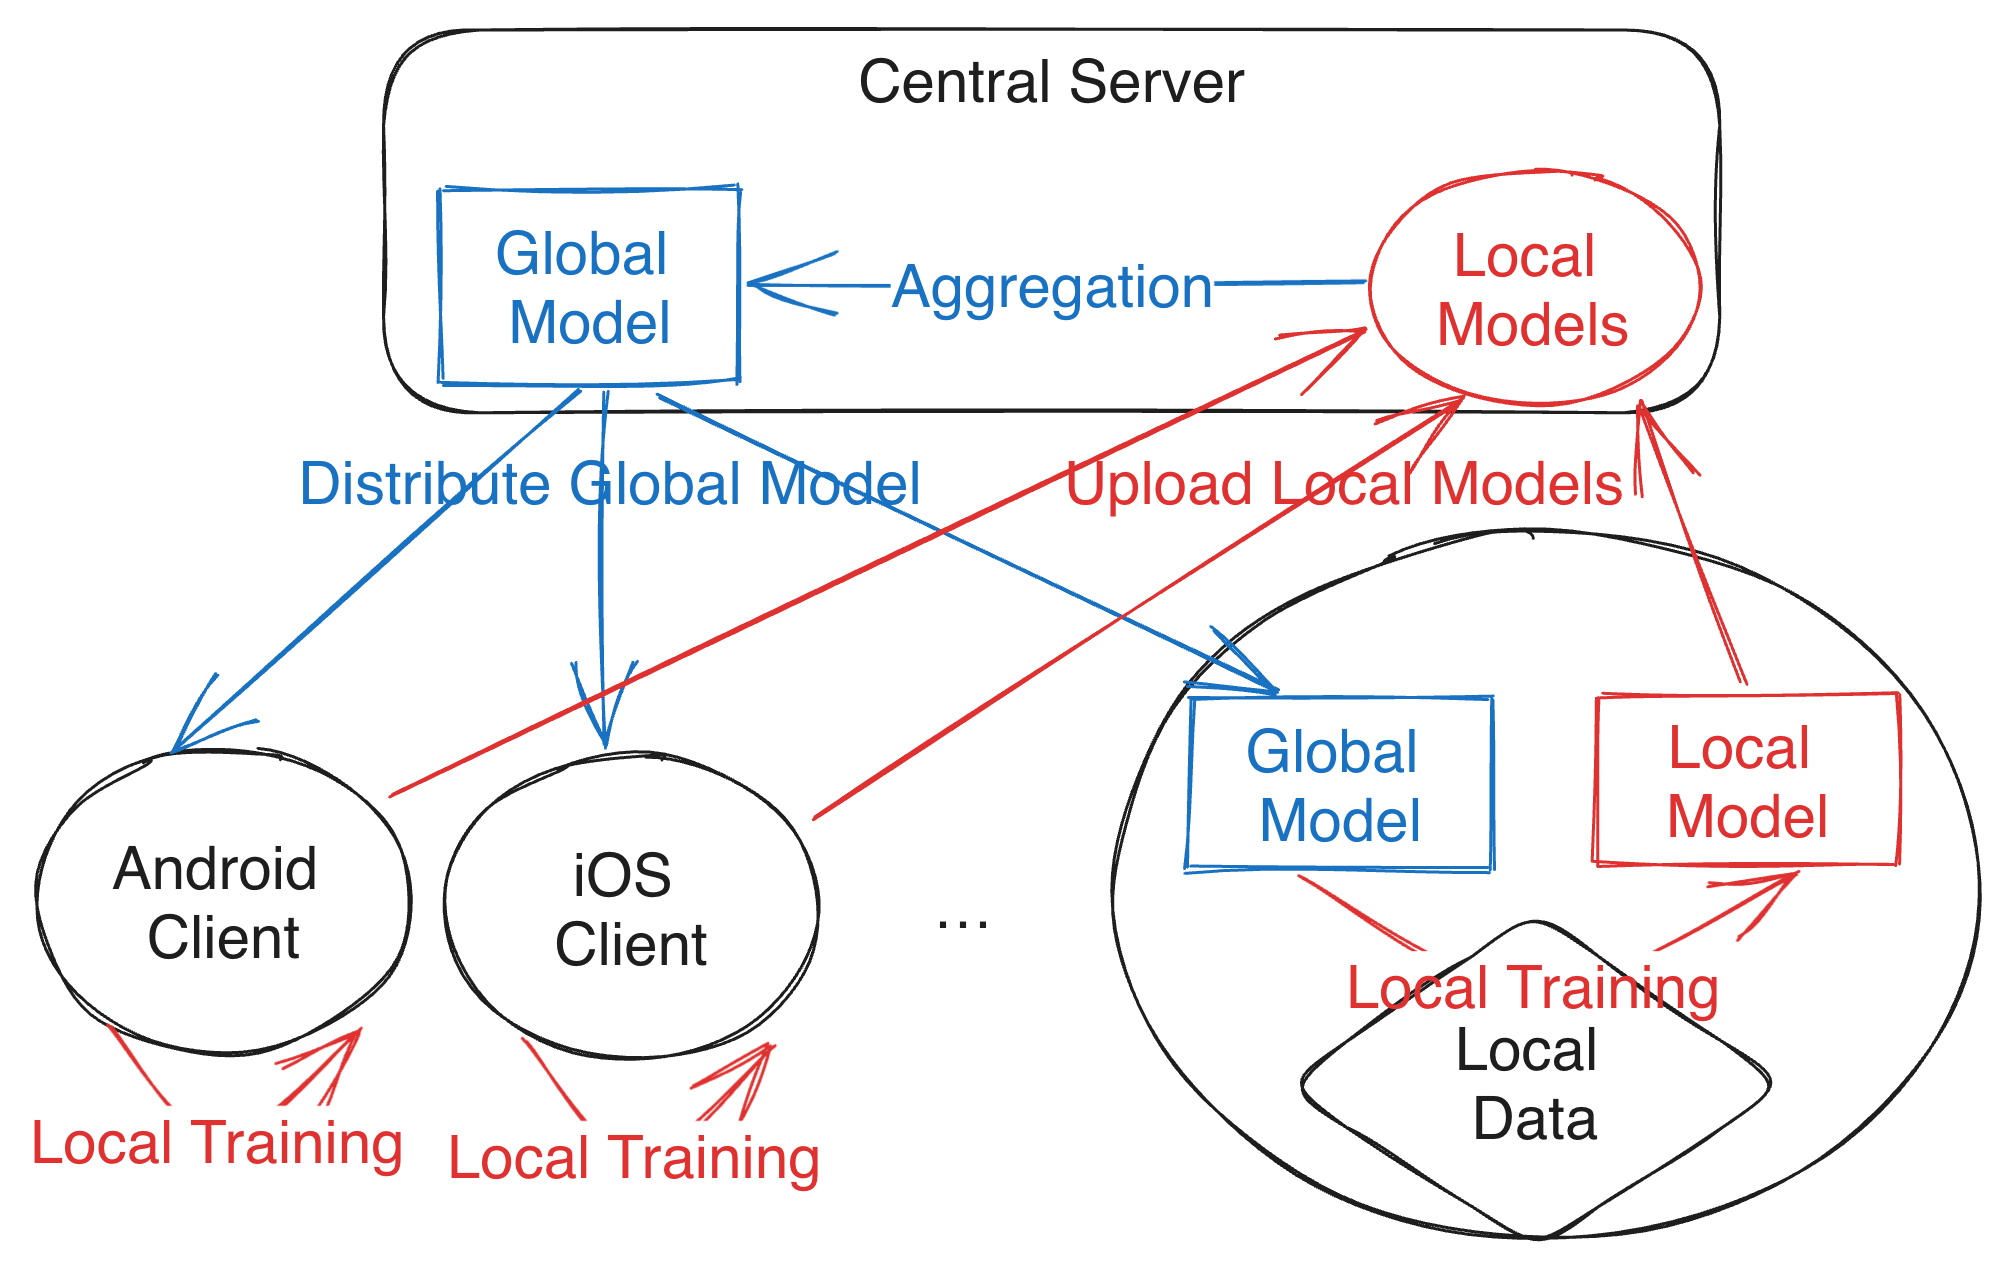
\includegraphics[width=0.7\textwidth]{general_fl.png}
    \caption{General Federated Learning Procedure on Smartphones.}
    \label{fig:general-fl}
\end{center}\end{figure}

The specific implementations of federated learning on mobile devices may vary,
but they share a common foundation. The FedAvg algorithm,
presented with federated learning itself~\cite{mcmahan2017communication},
stands as the most typical federated learning algorithm. In FedAvg,
a fixed number of $C$ out of $K$ clients are selected for local training in each
iteration.
The local training aims to minimize the loss $L$ of the model for each client's
local data partition $P_k (k \in \{1, 2, \dots, K\})$:
\begin{equation}
\min_{w_k} L(P_k;w_k),
\end{equation}
starting from the parameters $w^{(t)}$ of the latest global model from the
server, and scheduled for a fixed number of $E$ epochs.
To optimize the global model for the entire training dataset $\bigcup_k P_k$,
FedAvg aims to minimize the weighted average of local losses
\begin{equation}
\min_{w} \frac{\sum_k |P_k|L(P_k;w)}{\sum_k |P_k|},
\text{ where }|P_k|\text{ is the size of }P_k,
\end{equation}
by computing the weighted average of local models' weights
\begin{equation}
w^{(t+1)}=\sum_k \frac{|P_k|}{\sum_k |P_k|}w_k^{(t+1)}
\end{equation}
to update the global model.
This iteration is repeated until model convergence or experiment termination.
FedAvg has proven effective and practical in various experimental scenarios,
benchmarked against earlier algorithms in data center
settings~\cite{bonawitz2019towards}.

\section{Machine Learning Operations}

% TODO: Improve this and cite.
Machine learning operations (MLOps) is a set of practices similar to
development operations (DevOps).
In development operations,
the software development process and the deployment process are integrated,
so that new software changes made by the development team can be
automatically deployed into production.
Similarly, in machine learning operations,
changes in the machine learning algorithms can be automatically deployed into
production.
Machine learning operations is desirable when the development velocity on
the machine learning algorithms is high,
and feedbacks from the production environment are important to improve
the machine learning algorithms.
